\section{Kvocientni prostori}
\subsection{Kvocientna topologija}
\begin{definicija}
    Naj bo \(X\) množica, \(\sim\) ekvivalenčna relacija na \(X\). 
    \begin{itemize}
        \item Za poljuben \(x \in X\) označimo \([x] = \setb{y \in X}{y \sim x}\) \df{ekvivalenčni razred}, ki pripada \(x\).
        \item \df{Kvocientna množica} množice \(X\) po relacije \(\sim\) je množica vseh ekvivalenčnih razredov \(\setb{[x]}{x \in X} =: X/_\sim\).
        \item Preslikava \(q: X \to X/_\sim, \ q(x) = [x]\) je \df{kvocientna projekcija}.
    \end{itemize}    
\end{definicija}

\begin{opomba}
    Ekvivalenčni razredi predstavljamo kot točke.
\end{opomba}

\begin{primer}
    Naj bo \(X = [0, 1]\). Ekvivalenčna relacija \(\sim\) določna z \[0 \sim 1 \quad (1 \sim 0, \all{x \in X}x \sim x).\]
    Kako si lahko predstavljamo kvocientno množico \(X/_\sim\)? Bodisi kot interval \([0,1)\) bodisi kot krožnico.
    \begin{center}
        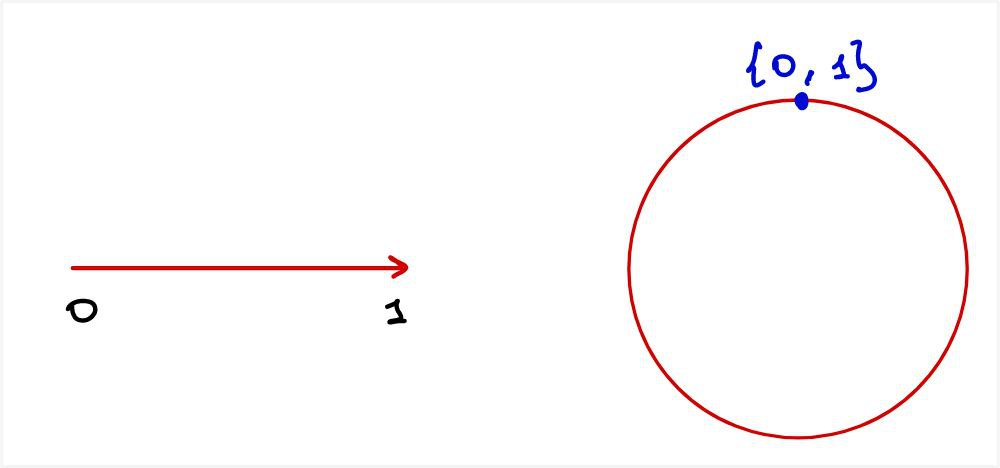
\includegraphics[width=0.5\textwidth]{img/01_001.jpg}      
    \end{center}
\end{primer}

\begin{opomba}
    \
    \begin{itemize}
        \item Pri opisu ekvivalenčne relacije bomo običajno navedli le netrivialne relacije, ki generirajo ekvivalenčno relacijo, ob upoštevanju lastnosti ekvivalenčnih relacij.
        \item Ekvivalenčna relacija \(\sim\) na \(X\) določa razdelitev množice \(X\) na ekvivalenčne razrede. To razdelitev označimo z \(\mathcal{R} = \setb{[x]}{x \in X} \subseteq P(X)\). Kvocientno množico lahko označimo z \(X/_\sim = X/_\mathcal{R}\).
        \item Če \(\sim\) določa le en netrivialen ekvivalenčni razred \(A \subseteq X, \ |A| \neq 1\), potem kvocientno množico označimo z \(X/_A\).
    \end{itemize}
\end{opomba}

Če je \(X\) topološki prostor in \(\sim\) ekvivalenčna relacija na \(X\), želimo \(X/_\sim\) opremiti z topologijo tako, da bo ta odražala lastnosti prostora \(X\). Posebej želimo, da je kvocientna projekcija \(q: X \to X/_\sim\) zvezna.

Pogoj \[\all{\op{V} \subseteq \qs{X}} \invimg{q}(V) \subseteq X \ \text{je odprta}\] topologije na \(\qs{X}\) ne določa enolično -- če neka topologija na \(\qs{X}\) temu ustreza, ustreza tudi vsaka šibkejša. Zato je \(\qs{X}\) smiselno opremiti z najmočnejšo topologijo, pri kateri je \(q\) zvezna. Torej za odprte množice v \(\qs{X}\) vzamemo vse, ki imajo odprte praslike v \(X\).

\begin{definicija}
    Naj bo \((X, \T)\) topološki prostor in \(\sim\) ekvivalenčna relacija na \(X\).
    \begin{itemize}
        \item \df{Kvocientna topologija} na \(\qs{X}\) je \[\T_\sim = \setb{V \subseteq \qs{X}}{\invimg{q}(V) \subseteq X \ \text{odprta}}.\]
    \end{itemize}
\end{definicija}

\begin{trditev}
    \(\T_\sim\) je topologija na \(\qs{X}\).
\end{trditev}

\begin{proof}
    Preverimo lastnosti.
\end{proof}

\begin{opomba}
    V kvocientni topologiji na \(\qs{X}\) velja:
    \[V \subseteq \qs{X} \ \text{je odprta} \liff \invimg{q}(V) \subseteq X \ \text{je odprta}.\]
    \((\Rightarrow)\) je zveznost preslikave \(q\);

    \((\Leftarrow)\) je največjost \(\T_\sim\).

    Velja tudi: 
    \[Z \subseteq \qs{X} \ \text{je zaprta} \liff \invimg{q}(Z) \subseteq X \ \text{je zaprta}.\]
\end{opomba}

\begin{primer}
    Ali je torej \(q\) odprta in zaprta? Ni nujno!
    \begin{itemize}
        \item Naj bo \(X = [0,1], \ \mathcal{R} = \set{[0, 1), \set{1}}\). Kaj je \(\q{X}{\mathcal{R}}\)? Ali sta \(\set{[0]}\) in \(\set{[1]}\) odprti? Ali je \(q\) zaprta?
        \item Naj bo \(X = [0,2], \ [1, 2] \ \text{edini netrivialni ekvivalenčni razred}\). Kaj je \(\q{X}{[1, 2]}\)? Ali je \(q\) odprta?
        \item Naj bo \(X = [0, 1], \ A = X \cap \Q, \ B = X \setminus \Q\). Kaj je \(\q{X}{\set{A, B}}\)? Kaj je kvocientna topologija?
    \end{itemize}
\end{primer}

\newpage
\begin{definicija}
    Naj bo \(X\) množica in \(\sim\) ekvivalenčna relacija. 
    \begin{itemize}
        \item Za \(A \subseteq X\) je njeno \df{nasičenje} enako \[\invimg{q}(\img{q}(A)) = \bigcup_{x \in A} [x] = \text{unija vseh ekvivalenčnih razredov, ki sekajo} \ A.\]
    \end{itemize}
\end{definicija}

\begin{trditev}
    Naj bo \(X\) topološki prostor, \(\sim\) ekvivalenčna relacija, \(A \subseteq X\). Velja:
    \begin{itemize}
        \item \(\img{q}(A) \subseteq \qs{X} \ \text{je odprta/zaprta} \liff  \text{nasičenje} \ \invimg{q}(\img{q}(A)) \ \text{odprto/zaprto}\). 
        \item \(\all{\op{U} \subseteq X} \invimg{q}(\img{q}(U)) \ \text{odprto/zaprto} \lthen q \ \text{je odprta/zaprta}\).
    \end{itemize}
\end{trditev}

\begin{proof}
    Definicija nasičenosti.
\end{proof}

\paragraph{Cilj} Imamo nek topološki prostor \(X\) in ekvivalenčno relacijo \(\sim\). Če je to mogoče, želimo poiskati nek geometrični model \(Y\) za kvocient \(\qs{X}\) in jasno pokazati, da je \(\qs{X} \approx Y\).

\begin{primer}
    \
    \begin{itemize}
        \item Naj bo \(X = \R, \ A = \Z\). Kaj je \(\q{\R}{A}\)?
        \item Naj bo \(X = [0,1], \ A = \setb{\frac{1}{n}}{n \in \N} \cup \set{0}\). Kaj je \(\q{\R}{A}\)? Ali je kompakten?
    \end{itemize}
    V obeh primerih imamo števno mnogo krožnic, spetih v eni točki. Ali sta ta prostora homeomorfna?
\end{primer}

\subsection{Kvocientne preslikave}
\paragraph{Cilj} Razumeti preslikave iz kvocientov.

Naj bo \(X\) topološki prostor, \(\sim\) ekvivalenčna relacija.

\[
    \begin{tikzcd}
        X \arrow[swap]{d}{q} \arrow{rd}{f \, := g \,  \circ \, q} &   \\%
        X/_\sim \arrow[swap]{r}{g} & Y
    \end{tikzcd}
\]

Zvezna preslikava \(g: \qs{X} \to Y\) določa zvezno preslikavo \(f = g \circ q: X \to Y\).

Če je \(x \sim y\) v \(X\), je \([x] = q(x) = q(y) = [y]\) in zato je \(f(x) = g(q(x)) = g(q(y)) = f(y)\). Torej ta \(f\) je konstantna na ekvivalenčnih razredih, tj. ekvivalentne točke slika v iste.

Želimo obratno: za preslikavo \(f: X \to Y\) poiskati pogoje, da določa preslikavo iz \(\qs{X}\) v \(Y\).
%
\[
    \begin{tikzcd}
        X \arrow{r}{f} \arrow[swap]{d}{q} & Y \\
        \qs{X} \arrow[dashed, swap]{ru}{\overline{f}}
    \end{tikzcd}
\]
%
Če naj diagram komutira, mora biti \(f\) konstantna na ekvivalenčnih razredih:
\[
    \all{x,y \in X} x \sim y \lthen f(x) = f(y).
\]

Če to velja, potem definiramo \[\overline{f}([x]) := f(x).\]
\(\overline{f}\) je preslikava, inducirana s \(f\).

\begin{trditev}
    Naj bo \(X\) topološki prostor, \(\sim\) ekvivalenčna relacija, \(f: X \to Y\) funkcija, ki je konstantna na ekvivalenčnih razredih. Potem \(f\) določa dobro definirano preslikavo \[\overline{f}: \qs{X} \to Y,\] za katero velja: \[\overline{f} \circ q = f.\]
    Poleg tega velja:
    \begin{itemize}
        \item Če je \(f\) zvezna, potem je tudi \(\overline{f}\) zvezna.
        \item Če je \(f\) surjektivna, je \(\overline{f}\) surjektivna.
        \item Če za \(\all{x, y \in X} x \not \sim y \lthen f(x) \neq f(y)\), potem je \(\overline{f}\) injektivna, tj. \(f\) loči ekvivalenčne razrede.
    \end{itemize}
\end{trditev}

\begin{proof}
    Definicija kvocientne topologije.
\end{proof}

\newpage
Zanima nas, kdaj bo \(\overline{f}\) homeomorfizem. Velja:

\(\overline{f}: \qs{X} \to Y\) je homeomorfizem, če 
\begin{itemize}
    \item zvezna, bijektivna in inverz zvezen oz.
    \item bijekcija iz \(\qs{X}\) v \(Y\) in porodi bijekcijo med topologiji na \(\qs{X}\) in \(Y\).
\end{itemize}
Torej NTSE
\begin{itemize}
    \item \(\overline{f}\) je homeomorfizem.
    \item \(\overline{f}\) je bijekcija iz \(\qs{X}\) v \(Y\) in porodi bijekcijo med odprtimi množici.
    \item \(\overline{f}\) je bijekcija in velja:    
    \begin{align*}
        \all{V \subseteq Y} V \ \text{je odprta} &\liff \invimg{\overline{f}}(V) \subseteq \qs{X} \ \text{je odprta (bijekcija med topologiji)} \\
        &\liff \invimg{q}(\invimg{\overline{f}}(V)) \ \text{je odprta (definicija kvociente topologije)} \\
        &\liff \invimg{f}(V) \subseteq X \ \text{je odprta (diagram komutira)}
    \end{align*}
\end{itemize}

\begin{definicija}
    Naj bosta \(X, Y\) topološka prostora in \(f: X \to Y\) funkcija. Če je \(f\) surjektivna in če 
    \[\all{V \subseteq Y} V \ \text{je odprta} \liff \invimg{f}(V) \subseteq X \ \text{je odprta},\]
    potem \(f\) imenujemo \df{kvocientna preslikava}.
\end{definicija}

\begin{opomba}
    \
    \begin{itemize}
        \item Po definiciji kvocientne topologiji, je kvocientna projekcija kvocientna preslikava. 
        
        Obratno: vsako kvocientno preslikavo \(f: X \to Y\) lahko obravnavamo kot kvocientno projekcijo pri ekvivalenčni relaciji, določeni z razbitjem \(X\) na praslike točk.
        \item Kvocientna preslikava je vedno zvezna, ni pa nujno odprta niti zaprta.
        \item Implikacija \((\Leftarrow)\) v definiciji je posebna lastnost, tej včasih rečemo \df{kvocientnost v ožjem smislu}.
        
        Za zvezno surjekcijo je za njeno kvocientnost potrebno preveriti le ta pogoj.
        \item Surjektivna funkcija \(f\) je kvocientna preslikava natanko tedaj, ko 
        \[\all{Z \subseteq Y} Z \ \text{je zaprta} \liff \invimg{f}(Z) \subseteq X \ \text{je zaprta}.\]
    \end{itemize}
\end{opomba}

\begin{lema}
    Naj bo funkcija \(f: X \to Y\) zvezna in surjektivna. Če je \(f\) odprta ali zaprta, je kvocientna.
\end{lema}

\begin{proof}
    Preveriti je treba le kvocientnost v ožjem smislu.
\end{proof}

\begin{izrek}[O prepoznavi kvocienta]
    Naj bosta \(X, Y\) topološka prostora in \(\sim\) ekvivalenčna relacija na \(X\). Naj bo \(f:~X~\to~Y\) kvocientna preslikava, ki naredi enake identifikacije kot \(\sim\), tj.\ \(f\) je konstantna na ekvivalenčnih razredih in loči ekvivalenčne razrede:
    \[\all{x, y \in X} x \sim y \liff f(x) = f(y).\]
    Potem je inducirana preslikava \(\overline{f}: \qs{X} \to Y\) homeomorfizem.
\end{izrek}

\begin{proof}
    Sledi iz izpeljave zgoraj.
\end{proof}

\begin{primer}
    Poišči podprostor kakega evklidskega prostora, ki mu homeomorfen kvocient:
    \begin{itemize}
        \item \([0,1]/_{\set{0, 1}}\)
        \item \([0,1] \times [0,1]/_\sim\), kjer \(\all{y \in [0,1]} (0, y) \sim (1, y)\)
        \item \([0,1] \times [0,1]/_\sim\), kjer \(\all{y \in [0,1]} (0, y) \sim (1, 1- y)\)
        \begin{opomba}
            Mobiusov trak lahko vložimo v \(S^1 \times B^2\): začnemo z daljico v \(B^2\) in jo vzdolž faktorja \(S^1\) zavrtimo za kot \(\pi\).
        \end{opomba}
        \item \([0,1] \times [0,1]/_\sim\), kjer \(\all{y \in [0,1]} (0, y) \sim (1, y)\) in \(\all{x \in [0,1]} (x, 0) \sim (x, 1)\)
        \item \(B^2/_{S^1}\)
        \item \((\text{I}^2 + \text{I}^2)/_\sim\), kjer \(\all{y \in [0,1]} \text{in}_1 (1, y) \sim \text{in}_2 (0, f(y))\), kjer je \(f: \text{I} \to \text{I}\) poljuben homomorfizem
    \end{itemize}
\end{primer}

\subsubsection*{Operacije s kvocientnimi preslikavami}
\begin{trditev}
    Naj bosta \(f: X \to Y\) in \(g: Y \to Z\) preslikavi.
    \begin{enumerate}
        \item Če sta \(f, g\) kvocientni, potem \(g \circ f\) kvocientna.
        \item Če je \(g \circ f\) kvocientna in sta \(f, g\) zvezni, potem je \(g\) kvocientna.
    \end{enumerate}
\end{trditev}

\begin{proof}
    Definicija kvocientne preslikave.
\end{proof}

\begin{opomba}
    1.\ točka nam pove, da lahko identifikacijo razdelimo na več delov.
\end{opomba}

\begin{trditev}
    Naj bo \(X\) topološki prostor in \(\sim_X\) ekvivalenčna relacija na \(X\). Naj bo \(f: X \to Y\) homeomorfizem, ki določa ekvivalenčno relacijo \(\sim_Y\) na \(Y\), usklajeno z \(\sim_X\), tj. 
    \[y_1 \sim_Y y_2 \liff f^{-1}(y_1) \sim_X f^{-1}(y_2),\]
    potem \[X/_{\sim_X} \approx Y/_{\sim_Y}\]
    %
    \[
        \begin{tikzcd}[column sep=2cm, row sep=1cm]
            X \arrow{r}{f} \arrow[swap]{d}{q_X} \arrow[draw=blue]{rd}{\textcolor{blue}{q_Y \circ f}} & Y \arrow{d}{q_Y} \\
            X/_{\sim_X} \arrow[dashed, swap]{r}{\overline{f}} & Y/_{\sim_Y}
        \end{tikzcd}
    \]
    %
\end{trditev}
\begin{proof}
    Preslikava \(q_Y \circ f\) je kompozitum dveh kvocientnih preslikav, torej je kvocienta. Torej je dovolj preveriti, da preslikava \(q_Y \circ f\) dela iste identifikacije kot \(\sim_X\).
\end{proof}

\begin{primer}
    Naj bo \(1 \in S^1 \subseteq \C \equiv \R^2\). Naj bo \(A = S^1 \times \set{1} \cup \set{1} \times S^1 \subseteq S^1 \times S^1 = \mathbb{T}\), kjer je \(\mathbb{T}\) \df{torus}. Kaj je \(T/_A\)?

    Ideja: Torus prerežemo vzdolž \(A\), da dobimo kvadrat z identifikacijami na robu.
\end{primer}

\subsection{Deljivost topoloških lastnosti}
\begin{definicija}
    Topološka lastnost \(\mathcal{L}\) je \df{deljiva}, če za vsak topološki prostor \(X \in \mathcal{L}\) in vsako ekvivalenčno relacijo \(\sim\) na \(X\) velja, da \(X/_\sim \in \mathcal{L}\).

    Ekvivalentno: Lastnost \(\mathcal{L}\) je deljiva, če se ohranja pro kvocientnih preslikavah.
\end{definicija}

\begin{trditev}
    Naj bo \(X\) topološki prostor in \(\sim\) ekvivalenčna relacija na \(X\). Velja:
    \[X/_\sim \in T_1 \liff \text{ekvivalenčni razredi so zaprti}.\]
\end{trditev}

\begin{proof}
    Karakterizacija \(T_1\) in definicija kvocientne projekcije.
\end{proof}

\begin{izrek}[Aleksandrov]
    Za poljuben metrični kompakt \(X\) obstaja zvezna surjekcija \(f: C \to X\)
\end{izrek}

\begin{opomba} \
    \begin{itemize}
        \item Cantorjeva množica \(C\) je popolnoma nepovezan metrični kompakt brez izoliranih točk (karakterizacija \(C\)).
        \item Taka \(f\) je kvocientna, saj je surjektivna, zvezna in zaprta, ker slika iz kompakta v \(T_2\) prostor.
        \item Dokaz tega izreka je zelo težek, ampak lahko eksplicitno zapišemo preslikavo iz \(C\) v \([0,1]\), npr. 
        \begin{align*}
            f: C &\longrightarrow  [0,1] \\
            \sum_{i=1}^{\infty} \frac{c_i}{3^i} &\longmapsto \sum_{i=1}^{\infty} \frac{c_i / 2}{2^i}, \ c_i \in \set{0, 2}
        \end{align*}
    \end{itemize}
\end{opomba}

\begin{trditev} \ 
    \begin{enumerate}
        \item Deljive so naslednje topološki lastnosti:
        \begin{itemize}
            \item Kompaktnost
            \item Povezanost (s potmi)
            \item Lokalna povezanost (s potmi)
            \item Separablinost
            \item Trivialnost, diskretnost
        \end{itemize}
        \item Nedeljive so naslednje topološki lastnosti:
        \begin{itemize}
            \item Separacijske: \(T_0 - T_4\)
            \item Lokalna kompaktnost
            \item \(1\)-števnost in \(2\)-števnost
            \item Metrizabilnost
            \item Popolna nepovezanost
        \end{itemize}
    \end{enumerate}
\end{trditev}

\begin{proof} \
    \begin{enumerate}
        \item Deljivost:
        \begin{itemize}
            \item Kompaktnost, povezanost (s potmi), separabilnost, trivialnost in diskretnost: se ohranjajo pri zveznih surjektivnih preslikavah.
            \item Lokalna povezanost (s potmi): Prostor je lokalno povezan \(\liff\) Komponente vsake odprte množice so odprte. 
        \end{itemize}
        \item Nedeljivost:
        \begin{itemize}
            \item \(T_0\): \(X=[0,1], \ A = X \cap \Q, \ B = X \setminus \Q \leadsto X/_{\set{A, B}}\)
            \item \(T_1\): \(X=[0,1], \ \mathcal{R} = \set{[0,1), \set{1}} \leadsto X/_\mathcal{R}\)
            \item \(T_2, \ T_3, \ T_4\), metrizabilnost: \(X = \R \times \set{0,1}\), \(\all{x > 0}(x, 0) \sim (x, 1) \leadsto X/_\sim\)
            \item \(1\)-števnost, \(2\)-števnost, lokalna kompaktnost: \(X=[0,1] \times \N\), \(A = \set{0} \times \N \leadsto X/_A\)
            \item Popolna nepovezanost: Izrek Aleksandrova \qedhere
        \end{itemize}
    \end{enumerate}    
\end{proof}